\documentclass[../Main.tex]{subfiles}

\begin{document}

\IfFileExists{NewCommands.tex}       {% Add new commands here.
%
% Use "providecommand" instead of "newcommand" since we
% want to include this file in all subfiles, and if we
% used newcommand it would report the error
% "Command xxx already defined"
%
%
\providecommand{\dmOT}{\Delta m^2_{\rm 12}}
\providecommand{\dmsolar}{\Delta m^2_{\rm solar}}
\providecommand{\dmatm}{\Delta m^2_{\rm atm}}
\providecommand{\dmTT}{\Delta m^2_{\rm atm}}
\providecommand{\dmsq}[1]{\Delta m^{2}_{#1}}
\providecommand{\thatm}{\Delta m^2_{\rm atm}}
\providecommand{\thTT}{\theta_{\rm 23}}
\providecommand{\sinsq}[1]{\sin^{2}(\theta_{#1})}
\providecommand{\sinsqOT}{\sin^{2}(\theta_{\rm 12})}
\providecommand{\sinsqsolar}{\sin^{2}(\theta_{\rm solar})}
\providecommand{\sinsqTT}{\sin^{2}(\theta_{\rm 23})}
\providecommand{\sinsqTwoTT}{\sin^{2}(2\theta_{\rm 23})}
\providecommand{\dcp}{\delta_{\rm CP}}

\providecommand{\gsim}{\gtrsim}
\providecommand{\lsim}{\lesssim}
\providecommand{\Enu}{\rm{E}_\nu}
\providecommand{\Emu}{\rm{E}_\mu}
\providecommand{\Ecasc}{\rm{E}_{\rm casc}}
\providecommand{\Lmu}{\rm{L}_\mu}
\providecommand{\Lnu}{\rm{L}_\nu}
\providecommand{\Thetamu}{\theta_\mu}
\providecommand{\cosThetamu}{\cos{\theta_\mu}}
\providecommand{\cosThetanu}{\cos{\theta_\nu}}
\providecommand{\Thetanu}{\theta_\nu}
\providecommand{\nue}{\nu_{\rm e}}
\providecommand{\numu}{\nu_\mu}
\providecommand{\nutau}{\nu_\tau}

\providecommand{\ket}[1]{|#1\rangle}

\providecommand{\ue}[1]{|U_{e #1}|}
\providecommand{\umu}[1]{|U_{\mu #1}|}
\providecommand{\utau}[1]{|U_{\tau #1}|}
\providecommand{\uesq}[1]{|U_{e #1}|^{2}}
\providecommand{\umusq}[1]{|U_{\mu #1}|^{2}}
\providecommand{\utausq}[1]{|U_{\tau #1}|^{2}}

\providecommand{\Nch}{${\rm N}_{\rm ch}\,$}
\providecommand{\Ndir}{${\rm N}_{\rm dir}\,$}
\providecommand{\Nstr}{${\rm N}_{\rm str}\,$}
\providecommand{\Aeff}{${\rm A}_{\rm eff}\,$}
\providecommand{\Veff}{${\rm V}_{\rm eff}\,$}
\providecommand{\VeffNS}{${\rm V}_{\rm eff}$}

\providecommand{\pe}{$p.e.$ }
}       {}
\IfFileExists{../NewCommands.tex}    {% Add new commands here.
%
% Use "providecommand" instead of "newcommand" since we
% want to include this file in all subfiles, and if we
% used newcommand it would report the error
% "Command xxx already defined"
%
%
\providecommand{\dmOT}{\Delta m^2_{\rm 12}}
\providecommand{\dmsolar}{\Delta m^2_{\rm solar}}
\providecommand{\dmatm}{\Delta m^2_{\rm atm}}
\providecommand{\dmTT}{\Delta m^2_{\rm atm}}
\providecommand{\dmsq}[1]{\Delta m^{2}_{#1}}
\providecommand{\thatm}{\Delta m^2_{\rm atm}}
\providecommand{\thTT}{\theta_{\rm 23}}
\providecommand{\sinsq}[1]{\sin^{2}(\theta_{#1})}
\providecommand{\sinsqOT}{\sin^{2}(\theta_{\rm 12})}
\providecommand{\sinsqsolar}{\sin^{2}(\theta_{\rm solar})}
\providecommand{\sinsqTT}{\sin^{2}(\theta_{\rm 23})}
\providecommand{\sinsqTwoTT}{\sin^{2}(2\theta_{\rm 23})}
\providecommand{\dcp}{\delta_{\rm CP}}

\providecommand{\gsim}{\gtrsim}
\providecommand{\lsim}{\lesssim}
\providecommand{\Enu}{\rm{E}_\nu}
\providecommand{\Emu}{\rm{E}_\mu}
\providecommand{\Ecasc}{\rm{E}_{\rm casc}}
\providecommand{\Lmu}{\rm{L}_\mu}
\providecommand{\Lnu}{\rm{L}_\nu}
\providecommand{\Thetamu}{\theta_\mu}
\providecommand{\cosThetamu}{\cos{\theta_\mu}}
\providecommand{\cosThetanu}{\cos{\theta_\nu}}
\providecommand{\Thetanu}{\theta_\nu}
\providecommand{\nue}{\nu_{\rm e}}
\providecommand{\numu}{\nu_\mu}
\providecommand{\nutau}{\nu_\tau}

\providecommand{\ket}[1]{|#1\rangle}

\providecommand{\ue}[1]{|U_{e #1}|}
\providecommand{\umu}[1]{|U_{\mu #1}|}
\providecommand{\utau}[1]{|U_{\tau #1}|}
\providecommand{\uesq}[1]{|U_{e #1}|^{2}}
\providecommand{\umusq}[1]{|U_{\mu #1}|^{2}}
\providecommand{\utausq}[1]{|U_{\tau #1}|^{2}}

\providecommand{\Nch}{${\rm N}_{\rm ch}\,$}
\providecommand{\Ndir}{${\rm N}_{\rm dir}\,$}
\providecommand{\Nstr}{${\rm N}_{\rm str}\,$}
\providecommand{\Aeff}{${\rm A}_{\rm eff}\,$}
\providecommand{\Veff}{${\rm V}_{\rm eff}\,$}
\providecommand{\VeffNS}{${\rm V}_{\rm eff}$}

\providecommand{\pe}{$p.e.$ }
}    {}
\IfFileExists{../../NewCommands.tex} {% Add new commands here.
%
% Use "providecommand" instead of "newcommand" since we
% want to include this file in all subfiles, and if we
% used newcommand it would report the error
% "Command xxx already defined"
%
%
\providecommand{\dmOT}{\Delta m^2_{\rm 12}}
\providecommand{\dmsolar}{\Delta m^2_{\rm solar}}
\providecommand{\dmatm}{\Delta m^2_{\rm atm}}
\providecommand{\dmTT}{\Delta m^2_{\rm atm}}
\providecommand{\dmsq}[1]{\Delta m^{2}_{#1}}
\providecommand{\thatm}{\Delta m^2_{\rm atm}}
\providecommand{\thTT}{\theta_{\rm 23}}
\providecommand{\sinsq}[1]{\sin^{2}(\theta_{#1})}
\providecommand{\sinsqOT}{\sin^{2}(\theta_{\rm 12})}
\providecommand{\sinsqsolar}{\sin^{2}(\theta_{\rm solar})}
\providecommand{\sinsqTT}{\sin^{2}(\theta_{\rm 23})}
\providecommand{\sinsqTwoTT}{\sin^{2}(2\theta_{\rm 23})}
\providecommand{\dcp}{\delta_{\rm CP}}

\providecommand{\gsim}{\gtrsim}
\providecommand{\lsim}{\lesssim}
\providecommand{\Enu}{\rm{E}_\nu}
\providecommand{\Emu}{\rm{E}_\mu}
\providecommand{\Ecasc}{\rm{E}_{\rm casc}}
\providecommand{\Lmu}{\rm{L}_\mu}
\providecommand{\Lnu}{\rm{L}_\nu}
\providecommand{\Thetamu}{\theta_\mu}
\providecommand{\cosThetamu}{\cos{\theta_\mu}}
\providecommand{\cosThetanu}{\cos{\theta_\nu}}
\providecommand{\Thetanu}{\theta_\nu}
\providecommand{\nue}{\nu_{\rm e}}
\providecommand{\numu}{\nu_\mu}
\providecommand{\nutau}{\nu_\tau}

\providecommand{\ket}[1]{|#1\rangle}

\providecommand{\ue}[1]{|U_{e #1}|}
\providecommand{\umu}[1]{|U_{\mu #1}|}
\providecommand{\utau}[1]{|U_{\tau #1}|}
\providecommand{\uesq}[1]{|U_{e #1}|^{2}}
\providecommand{\umusq}[1]{|U_{\mu #1}|^{2}}
\providecommand{\utausq}[1]{|U_{\tau #1}|^{2}}

\providecommand{\Nch}{${\rm N}_{\rm ch}\,$}
\providecommand{\Ndir}{${\rm N}_{\rm dir}\,$}
\providecommand{\Nstr}{${\rm N}_{\rm str}\,$}
\providecommand{\Aeff}{${\rm A}_{\rm eff}\,$}
\providecommand{\Veff}{${\rm V}_{\rm eff}\,$}
\providecommand{\VeffNS}{${\rm V}_{\rm eff}$}

\providecommand{\pe}{$p.e.$ }
} {}


\graphicspath{{figures/}{DataAnalysis/figures/}}


\section{Data analysis}

The method to measure neutrino oscillations followed in this work is to compare the data with simulation templates. The parameters in the simulation are varied and the set that is most likely to explain the data is taken. The simulation is done by reproducing the interaction and detection steps, as described in Chapter \ref{ch:measurement}, and then passing the events through the same analysis as the data. The resulting events are used to fill a two-dimensional histogram with the reconstructed energy and zenith angle on the axes. The performance of the reconstructions varies depending on the true parameters of the neutrino, and reproducing them in full in the simulation is the most straight-forward way of correctly accounting for them.

\subsection{Statistical method}
The general method used to determine the oscillation parameters that the data favor is the binned maximum likelihood in the presence of nuisance parameters \cite{llh}. The two observables that modify the effect are the neutrino energy and the travel distance, while the two physical parameters of interest are the mixing angle $\theta_{23}$ and the mass difference $|\Delta m_{32}^2|$. A full calculation of oscillation probabilities is done using the Prob3++ software [reference].

The likelihood used for the fit is composed of a Poisson and a Gaussian term, as
\begin{equation}
\mathcal{L}(\lambda, x, w ; \mu, \sigma) = \prod_{i=1}^n \frac{\lambda_i^{x_i}e^{-\lambda_i}}{x_i\!}\;\prod_{j=1}^m \frac{1}{\sqrt{2 \pi \sigma^2_j}} e^{-\frac{(w_j - \mu_j)^2}{2\sigma^2_j}}.
\label{eq:PoissonLikelihood}
\end{equation} 
The Poisson term contains the probability for the prediction $\lambda_i$ of a particular simulation set to explailn the data $x_i$ in the $i$-th bin is calculated. The probabilities are multiplied, returning a value that can be compared with different $\lambda_i$ hypotheses. The nuisance parameters included, denoted by the subscript $j$, enter in the Gaussian term. They appear because the simulation depends on their mean values $\mu$, which are known to a precision $\sigma$ which can be insufficient for our purposes. Their true value, however, is of no interest for this study. We account for them by allowing the hypotheses on their value $w$ to change, penalizing their deviation from their mean value in units of their uncertainty.

The expression of Eq.\,\ref{eq:PoissonLikelihood} can be simplified by taking its logarithm. Also, since we are interested in comparing hypotheses, the absolute value of the likelihood is irrelevant, and constant factors can be eliminated. The simplified equation is then given by
\begin{equation}
LLH = \sum_{i=1}^n x_i \ln \lambda_i(\vec{\vartheta}, \vec{w}) - \lambda_i(\vec{\vartheta},\vec{w}) - \frac{1}{2} \sum_{j=1}^m  \frac{(w_j - \mu_j)^2}{\sigma^2_j}\,.
\label{eq:LLH}
\end{equation}
Here the same notation is used, with the exception that the dependence of the prediction on the oscillation parameters $\vec{\vartheta}$ and the nuisance parameters $\vec{w}$ is explicitly shown. Each of the events that end up in one of the bins of the histogram are weighted by the oscillation and nuisance parameters before they are summed up.

\textbf{Modify this section to include both the chi2 description together with the LLH. Chi2 can be described after the LLH as the approximation when you have enough stats per bin, plus you need fully uncorreltaed errors}

In the limit of high statistics, the log-likelihood function can be well approximated by a gaussian, turning Eq.~\ref{LLH} into something similar to a $\chi^2$ function. This function has the feature of isolating the uncorrelated errors in the denominator. It is therefore possible to include in a straightoforward manner the statistical error on the simulation available, as well as the statistical and systematic uncertainty on the estimation of the main background source, atmospheric muons. The fitting function used is then

\textbf{insert function and discuss the parameters}

\subsubsection{Data binning}
The flux diminishes with energy. Because of this the histogram is binned in the logarithm of the estimated energy $\log_{10}(E_\mathrm{reco}/\mathrm{GeV})$. As the effect from oscillations depends on travel distance, and this is proportional to the cosine of the zenith angle (see Eq.\,\ref{eq:propDistance}), the binning is done in $\cos\theta_\mathrm{reco}$.


\textbf{This is no longer true for all studies - need input from all}

Since the likelihood makes use of Poisson statistics, there is no minimum number of events per bin required. A finer binning allows to see more details of the data, but increases the number of calculations required to perform a fit. The effects on the sensitivity for using different number of bins were tested in a simulation sample, were it was found that after 8 bins the gain in sensitivity is marginal. Therefore, 8 bins are used for both axes.

\textbf{Discuss how the binning is roughly defined. Use resolution as guideline, discuss where the effect lives}

\subsubsection{Minimization}
The only remaining step is to maximize Eq.\,\ref{eq:LLH} and thus find the parameters $\vec{\vartheta}$ and $\vec{w}$ that describe the data best. In order to properly do so, it is necessary to continuously modify the parameters involved and obtain new predictions for the mean values at each bin, $\lambda_i$. Because of the number of variables involved, the MINUIT computational package \cite{minuit} was used for the task. The program performs a smart scan of the parameter space, and returns a set of values which yield the maximum likelihood that could be found. 

\subsection{Confidence regions}

\textbf{Section needs to be split between std. oscillations and ordering studies}

The precision of the measurement is determined by studying how much the likelihood changes as a function of the variables of interest in the vicinity of the best fit. When the fit is performed on variables that have no physical boundaries and no priors, the Wilks' theorem \cite{wilks} shows that it is possible to assume that the distribution of the log-likelihood difference,
\begin{equation}
LLH_\mathrm{diff} = -2\,\left(LLH_\mathrm{fit} - LLH_\mathrm{alt}\right)\,,
\end{equation}
 between the best fit and an alternative point near it follows a $\chi^2$ distribution, with a number of degrees of freedom that corresponds to the difference of the number of parameters fitted for both tests.

Once the map of likelihood values has been obtained the likelihood ratio is trivial to calculate. However, the problem being addressed in this analysis does not strictly fulfill the requirements of Wilks' theorem: there are physical limits to the values that some of the quantities can take, and prior knowledge is being enforced on some of the nuisance parameters. Whether the $LLH_\mathrm{diff}$ follows a $\chi^2$ distribution has to be tested.

Figure \ref{fig:llhratio} shows the $LLH_\mathrm{diff}$ distribution of pseudo-experiments, compared with the $\chi^2$ distribution expected to describe them. Two situations are shown: ruling out the case of no oscillations and determining the confidence regions if certain oscillation parameters are measured.
\begin{itemize}
\item In the left panel, the pseudo-experiments are drawn from a sample that does not contain oscillations. No oscillations is the null hypothesis; the alternate hypotheses allow for oscillation parameters to be fit. The distribution follows a $\chi^2$ with two degrees of freedom, thus Wilks' theorem is valid. 

\item The pseudo-experiments for the right panel are drawn from a sample that contains oscillations, calculated using the best known paremeters of Table \ref{table:CurrentOscParams}. The null hypothesis is given by the input oscillation parameters, while the alternate hypotheses are obtained by fitting their values. As it can be seen in the Figure, the pseudo-experiments are not described by a $\chi^2$ function with two degrees of freedom, but seem to fall in between the distributions given by a $\chi^2$ with one and two degrees of freedom.
\end{itemize}

\begin{figure}[h]
 \centering
 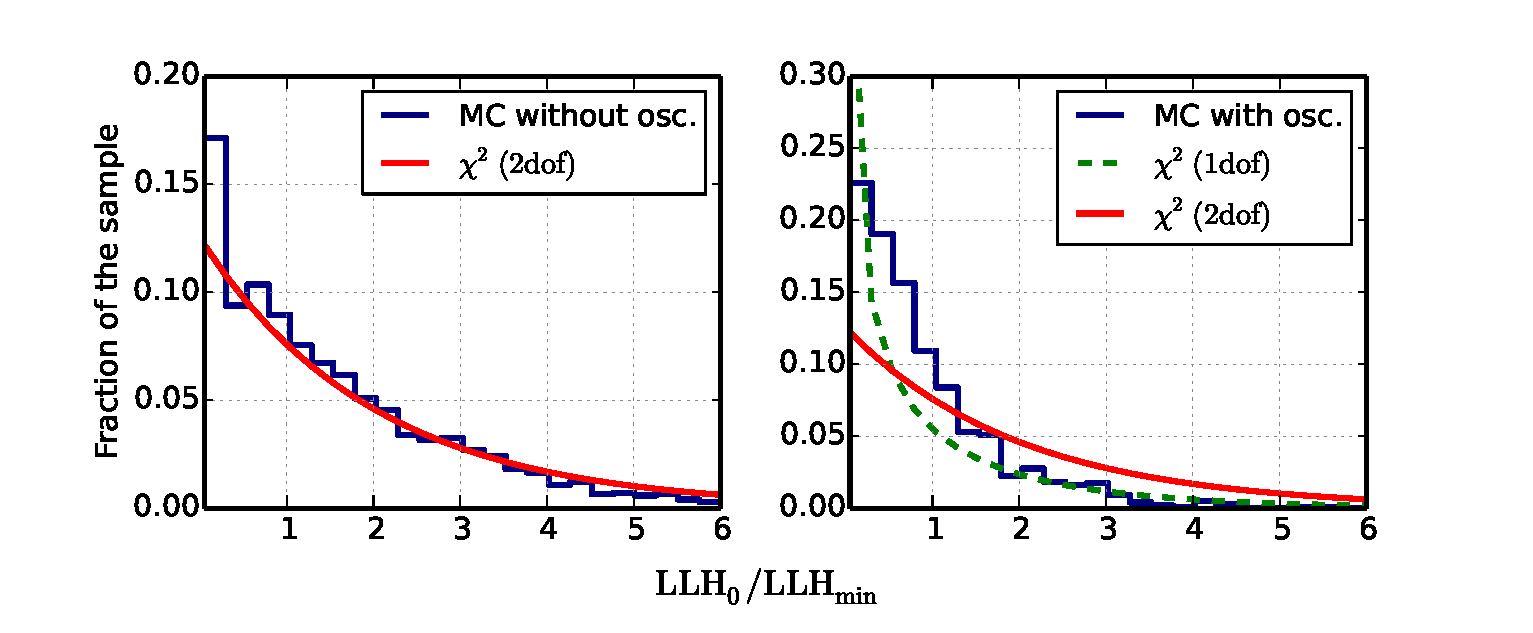
\includegraphics[width=0.9\textwidth]{chi2_distribution}
 \caption[Distribution of the test statistic.]{Distribution of the test statistic for 1000 pseudo-experiments. The distribution of the test statistic is compared with a $\chi^2$ distribution. Description in the text.}
 \label{fig:llhratio}
\end{figure}

Using the $LLH_\mathrm{diff}$ yields confidence regions which are bigger than they should be in certain regions. There are other alternatives for obtaining the confidence regions, which correctly deal with this type of situations, such as the one proposed by Feldman and Cousins \cite{feldmancousins}. However, they are computationally expensive as they require comparing the test statistic distribution of pseudo-experiments at each point of interest in the parameter space. As the $LLH_\mathrm{diff}$ over-estimates the errors, and it has been used by other experiments measuring the same effects \cite{minos1, t2k_disappearance}, it is used to obtain the final result.

\textbf{We have now used Feldman-Cousins for the latest result. We should estimate that}




\subsection{Including systematic uncertainties in the fit}
\label{sec:sys_uncertainties}
The effect of systematic uncertainties, with the exception of one to be discussed later, is accounted for by associating each source of error with a nuisance parameter, presented next. The energy-zenith angle distribution of the simulation depends on the value that the nuisance parameters take, and they are included in the maximization of the likelihood. The set of nuisance parameters can acquire any possible combination of values, which automatically takes correlations and degeneracies into account. Parameters with prior knowledge include a Gaussian term to the likelihood, as shown in Eq.\,\ref{eq:LLH}. If there is no prior information about the parameter, no such term is added.

The sources of uncertainty that are included in the study are those related to the flux and the ones connected to the detection process. They are listed in Table \ref{table:nuisance_list}, together with their allowed range and/or prior.
\begin{table}[h]
\caption[Systematic uncertainties included in the analysis.]{List of systematic uncertainties included in the analysis as nuisance parameters with their corresponding ranges and priors.}
\centering
\begin{Tabular}[1.2]{lcc}
\hline Nuisance parameter & Prior \\
\hline
Atm. $\mu$ contamination & up to 10\% \\ 
Atm. $\nu$ flux     & None \\ 
Atm. $\nu_e/\nu_\mu$   & $\sigma=20\%$ \\ 
Spectral index from \cite{honda06}     & $\sigma=0.05$ \\ 
Photo collection efficiency  & $\sigma=10\%$ \\ 
Efficiency increase of HQE DOMs & $\sigma=3\%$ \\ 
Scattering in ice columns [1/cm] & $\sigma=0.02$ \\ 
Bulk ice properties & See \cite{ice2} \\
\hline
\end{Tabular}
\label{table:nuisance_list}
\end{table}

With the exception of the last item listed, the uncertainties are a function of a single variable. The value of this variable can be modified each time that the likelihood is calculated, allowing for a continuous minimization. The inclusion of the top four, related to the flux, implies modifying the relative weight of the events in the sample. The next three, on the other hand, are related to the detection process, and any change in their values would require resimulating all events. Since this is technically hard to achieve, a different approach was taken, where only simulations of parameter changes in discrete steps are required.

\subsubsection{Parametrizing detection uncertainties}
The number of photons $N_{\gamma}$ that a DOM detects can be expressed as
\begin{equation}
N_\gamma = f\cdot g \cdot h \cdot N_0\,,
\label{eq:dom_n}
\end{equation}
where $N_0$ is the number of photons starting right outside the ice column traveling in the direction of the DOM. The functions $f$, $g$ and $h$ describe the overall efficiency of the IceCube DOMs, the relative efficiency between IceCube and DeepCore DOMs, and the optical properties of the ice column where the DOM sits, respectively. This formula is exact for photons only, but an approximation can be drawn from it for the case of full events.

Taking a reference simulation, variations are produced in which only one of the effects is changed. The sets are interpolated afterwards. The interpolation cannot be done on an event-by-event basis, as intrinsic variations and threshold effects will add and remove events from the sample. Instead, the interpolations are done on the bin contents of the histogram of observables.

The two-dimensional histogram used for the final analysis of the data has to be calculated for each simulation set. This means that all sets have to be put through the same analysis steps as the baseline simulation. During the fitting procedure, any change to the reference simulation, like a modification of the mixing angle, needs to be performed also on all the other simulation sets.

Once the changes to all sets have been made, the two-dimensional histogram used for the analysis is populated. One histogram is required for each simulation set. For each of the bins, a polynomial function $F$ is found, which describes the change in counts as a function of the variation introduced. As in Eq.\,\ref{eq:dom_n}, $F$ depends on the overall efficiency of the DOM. Figure \ref{fig:sys_discrete} demonstrates how a fit for $F$ is obtained for the effects of variations in the DOM efficiency in a particular bin.

\begin{figure}[h]
 \centering
 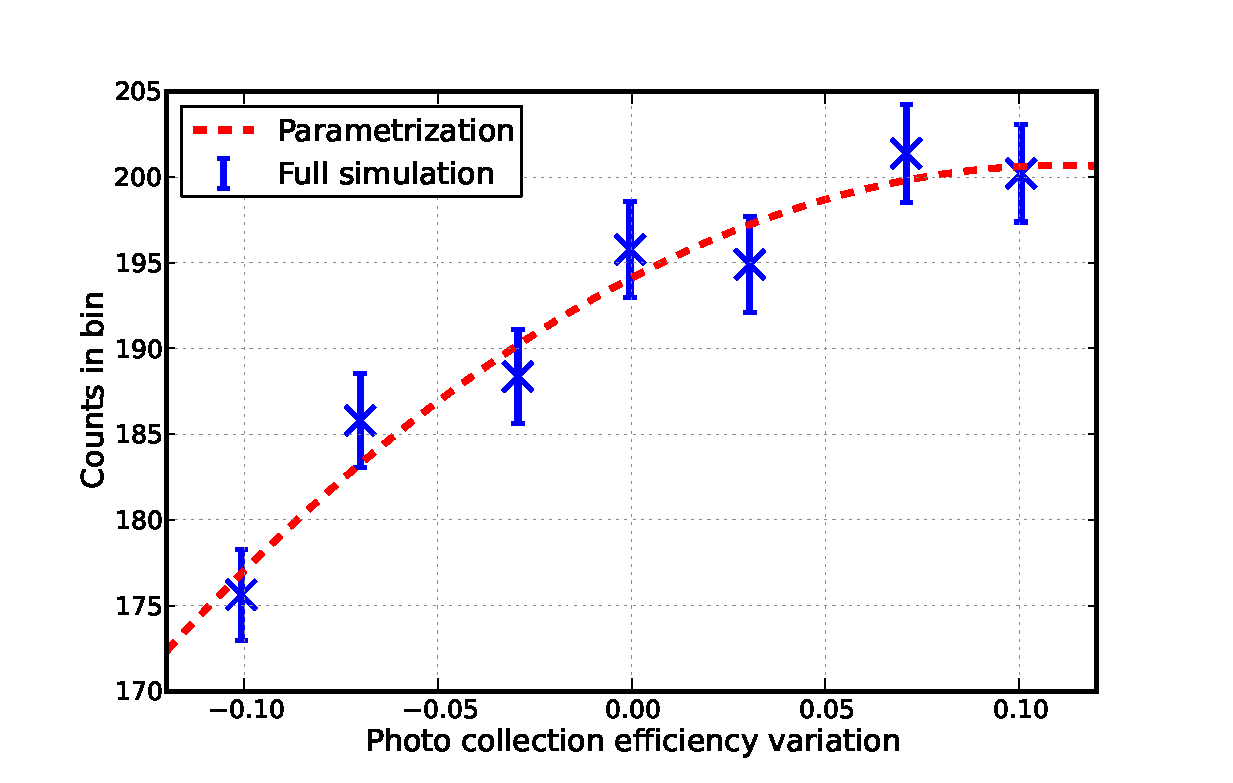
\includegraphics[width=0.6\textwidth]{DOMparam}
 \caption[Parametrization of discrete simulation sets.]{Fit of the impact of a given variation, light yield in this particular case, on the number of events in the $i$-th bin.}
 \label{fig:sys_discrete}
\end{figure}

The functions $G$ and $H$, for relative efficiency and angular acceptance, can be determined in the same way as the DOM efficiency. The number of events in the $i$-th bin of the energy-zenith angle histogram is then given by
\begin{equation}
N_i = F_i \cdot G_i\cdot H_i \cdot N_{i,\mathrm{baseline}}\,.
\end{equation}

Because of how the functions are defined, the formulation assumes that each detector effect can be parameterized and applied independently. According to simulation tests, the assumption is valid. The scheme presented can reproduce the results of full simulations with good accuracy.


\subsubsection{Accounting for discrete optical descriptions of the medium}
\textbf{We have done nothing in this part so far. The best we can do is test discrete models and check if our conclusions change, but we don't really ``account'' for them}

\textbf{[This is how we do all our diffuse fits at the moment. Is it worth it to describe it in detail? The section neglects things like point source studies (like Dark Matter searches) with DeepCore]}

\end{document}
